\chapter{Implementarea Software pe Modulul NodeMCU ESP8266 și platforma Blynk}
\thispagestyle{pagestyle}

În acest capitol este prezentat modul în care modulul NodeMCU primește datele de la placa de dezvoltare Arduino Mega și le transmite prin WiFi către platforma Blynk.

NodeMCU este o placă de dezvoltare ce are incorporat un modul ESP8266 de WiFI și chip de conversie USB CH340 \cite{nodemcu_ard}. Aceasta este programabilă utilizând Arduino IDE și acceptă același limbaj de programare bazat pe C++ folosit și de Arduino Mega.

Modulul ESP8266 oferă o soluție ideală pentru proiectele ce includ sistemele încorporate, oferind o conexiune facilă la WiFi. Acesta este comandat de o unitate centrală de procesare (CPU) Tensilica L106. Acest procesor dispune de o arhitectură pe 32 de biți de tip RISC ce poate ajunge până la o frecvență de 160 MHz, dar în același timp să și rămână eficient din punct de vedere al consumului\cite{nodemcu_datasheet}.

\section{Recepția datelor de la Arduino Mega}

Modulul NodeMCU primește datele de placa Arduino Mega prin intermediul comunicării seriale. Sunt folosiți pinii predefiniți de interfață UART
RX și TX. Această conexiune nu trebuie definită în cod deoarece s-a executat deja hardware conectând fire între cele două interfețe UART.

Pentru a inițializa conexiunea serială, în secțiunea \texttt{setup()} este apelată funcția \texttt{Serial.begin(9600)}. Argumentul \texttt{9600} este folosit pentru a seta rata de transfer (Baud Rate) și este identică cu cea setată pe Arduino Mega pentru a nu exista erori în transmisie.

\begin{code}[H]
\begin{lstlisting}[language=C++]
if (Serial.available()) {
    String line = Serial.readStringUntil('\n');
    float valuesFromSen[7]; 
    int start = 0;
    for (int i = 0; i < 7; i++) {
      int spaceIndex = line.indexOf(' ', start);
      if (spaceIndex == -1) spaceIndex = line.length(); // cand nu mai sunt spatii merge pana la sfrasit
      String subStr = line.substring(start, spaceIndex);
      valuesFromSen[i] = subStr.toFloat();
      start = spaceIndex + 1;
    }
\end{lstlisting}
\caption{Decodarea șirului primit de la Arduino Mega}
\label{code:decode_data_esp}
\end{code}

Primul pas în decodarea datelor trimise este citirea de pe interfața serială. Acest lucru se întâmplă la linia \textit{(1)} unde este verificat dacă interfața este disponibilă. Apoi, dacă aceasta este activă, se citesc date folosind funcția \texttt{Serial.readStringUntil('\textbackslash n')} până la înâlnirea caracterului \texttt{\textbackslash n}, iar datele citite sunt stocate în variabila \texttt{line} de tip șir de caractere. Datele primite sunt formatate astfel încât să fie despărțite printr-un caracter "spațiu" (' '), iar setul de date să se termine cu \texttt{\textbackslash n}, astfel se poate identifica momentul în care sunt trimise date noi.

Vectorul \texttt{valuesFromSen[7]} are o dimensiune de 7 elemente deoarece sunt trimise 7 valori aparținând senzorilor de pe placa Arduino Mega. Variabila \texttt{start} este folosită pentru a înregistra indexul de început al porțiunii ce este decodată.

La linia \textit{(5)} din Fragmentul \ref{code:decode_data_esp} se găsește o bulcă \texttt{for} ce este iterată de 7 ori pentru fiecare valoare ce trebuie decodată. În variabila \texttt{spaceIndex} va fi rețiuntă poziția caracterului spațiu găsit în șirul de caractere \texttt{line} începând de la poziția indicată de \texttt{start}. Dacă nu este găsit niciun caracter spațiu, \texttt{indexOf} va returna -1, ceea ce înseamnă că am ajuns la ultima valoare de decodat și setăm \texttt{spaceIndex} cu lungimea șirului.

Astfel, folosind indexul caracterului spațiu și indexul de start al subșirului, este extrasă porțiunea ce conține o valoare transmisă și se stochează în șirul de caractere \texttt{subStr} folosind funcția \texttt{substring()}. Porțiunea extrasă este apoi convertită în număr real și stocată în vectorul \texttt{valuesFromSen[7]}, iar variabila \texttt{start} este setată la următoare poziție după \texttt{spaceIndex} pentru a continua decodarea.

\section{Configurarea interfeței de afișare pe platforma Blynk}
\label{configurare_blynk}
Pentru a trimite date către platforma Blynk, este necesar să creăm un template pe platformă alegând un nume, modulul folosit și tipul de conexiune.

\begin{figure}[H]
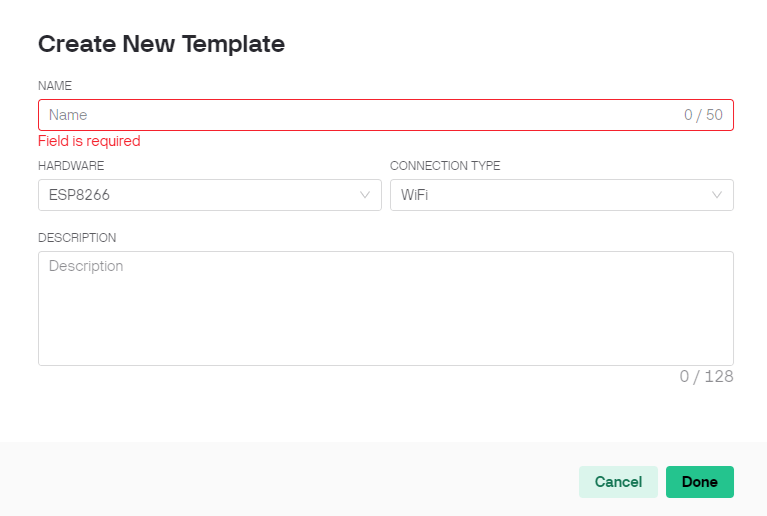
\includegraphics[width=0.7\linewidth]{bachelors_ro/images/blynk_template.png}
\caption{Crearea unui template pe platforma Blynk \cite{templ_blynk}}
\label{fig:template_blynk}
\end{figure}

După ce template-ul a fost creat, trebuie setate data stream-urile. Acestea reprezintă pini virtuali unde sunt transmise datele de pe modulul NodeMCU către platforma și sunt stocate individual. Acești pini pot fi configurați setând tipul de date primit și valoarea maximă ce poate fi reținută. Acest aspect este prezentat în Figura \ref{fig:data_stream_blynk}.

\begin{figure}[H]
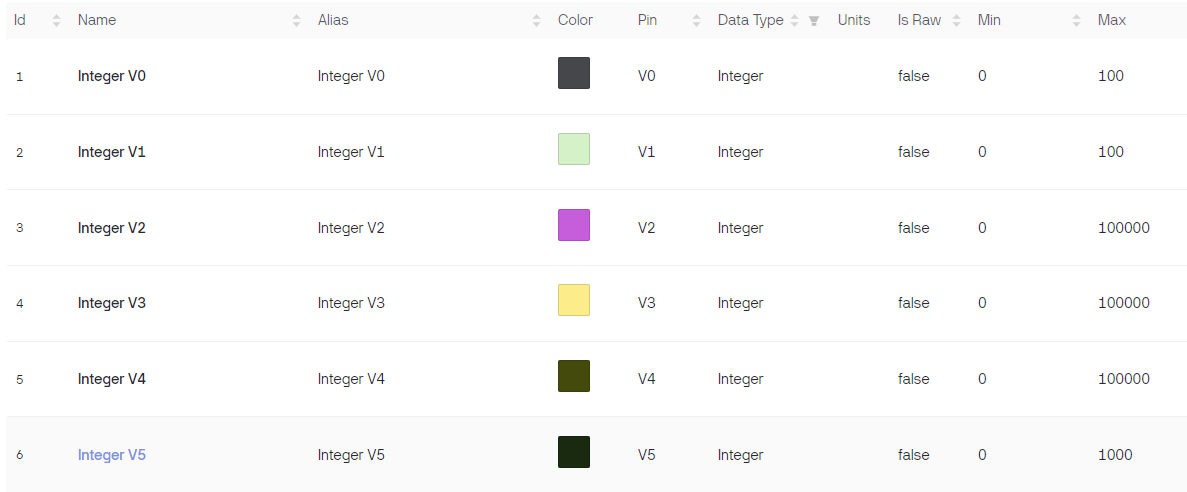
\includegraphics[width=0.9\textwidth, height=0.4\textwidth]{bachelors_ro/images/data_streams_blynk.png}
\caption{Configurarea data stream-urilor pe platforma Blynk \cite{templ_blynk}}
\label{fig:data_stream_blynk}
\end{figure}

Odată ce există un mod de recepționare a datelor pe platformă trebuie creată o interfață pentru a fi afișate. Astfel în secțiunea "Web Dashboard" pot fi adăugate elemente grafice ce afișează datele de la pinii virtuali. Platforma Blynk dispune de o varietate de widget-uri de afișaj, dar pentru acest proiect a fost ales widget-ul de tip indicator ("Gauge").

Acest gauge trebuie configurat la rândul său conform Figurii \ref{fig:config_gauge}. Trebuie să introducem un nume pentru widget și să alegem pinul virtual de la care acesta afișează datele.

\begin{figure}[H]
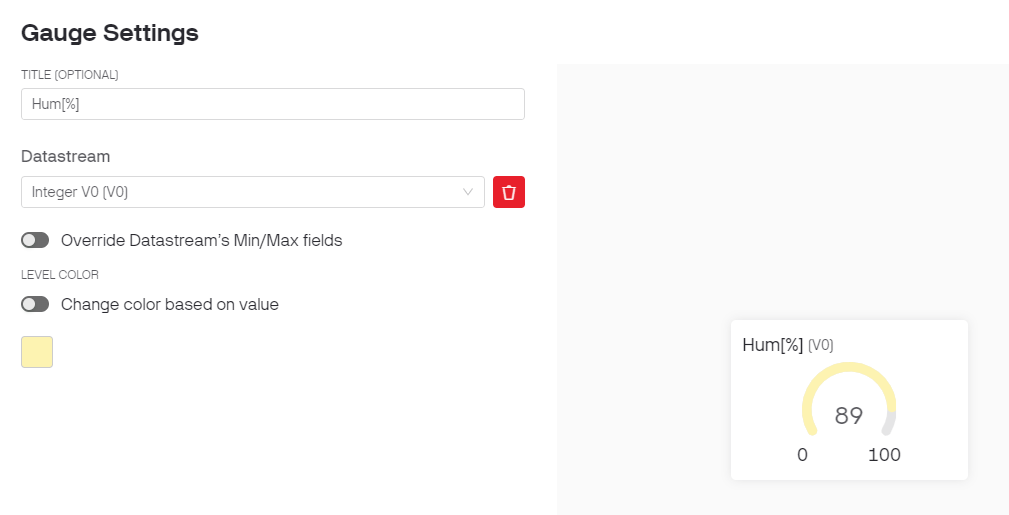
\includegraphics[width=0.8\linewidth]{bachelors_ro/images/config_gauge.png}
\caption{Configurarea gaguge-ului pentru un anumit pin virtual\cite{templ_blynk}}
\label{fig:config_gauge}
\end{figure}

După configurarea mai multor widget-uri pentru fiecare valoarea trimisă de modulul NodeMCU, în secțiunea "Devices" se poate observa interfața web finală obținută. (\ref{fig:interfata_blynk}).

\begin{figure}[H]
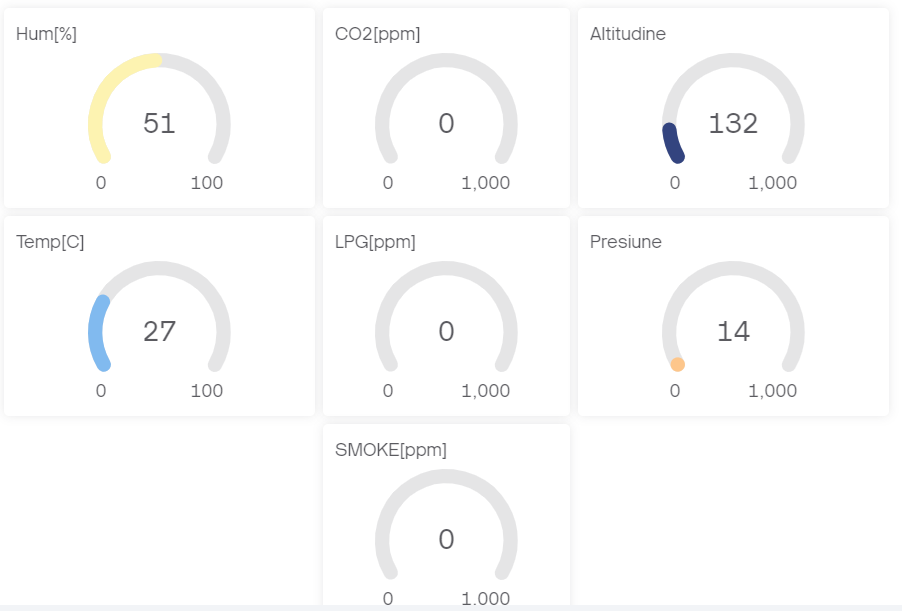
\includegraphics[width=0.7\linewidth]{bachelors_ro/images/interfata_blynk.png}
\caption{Interfața Web Blynk \cite{templ_blynk}}
\label{fig:interfata_blynk}
\end{figure}

Pentru a crea interfața mobile folosind aplicația Blynk sunt urmăriți aceeași pași menționați anterior. Interfața de pe platforma mobile Blynk se poate observa în Figura \ref{fig:interfata_blynk_mobile}.

\begin{figure}[H]
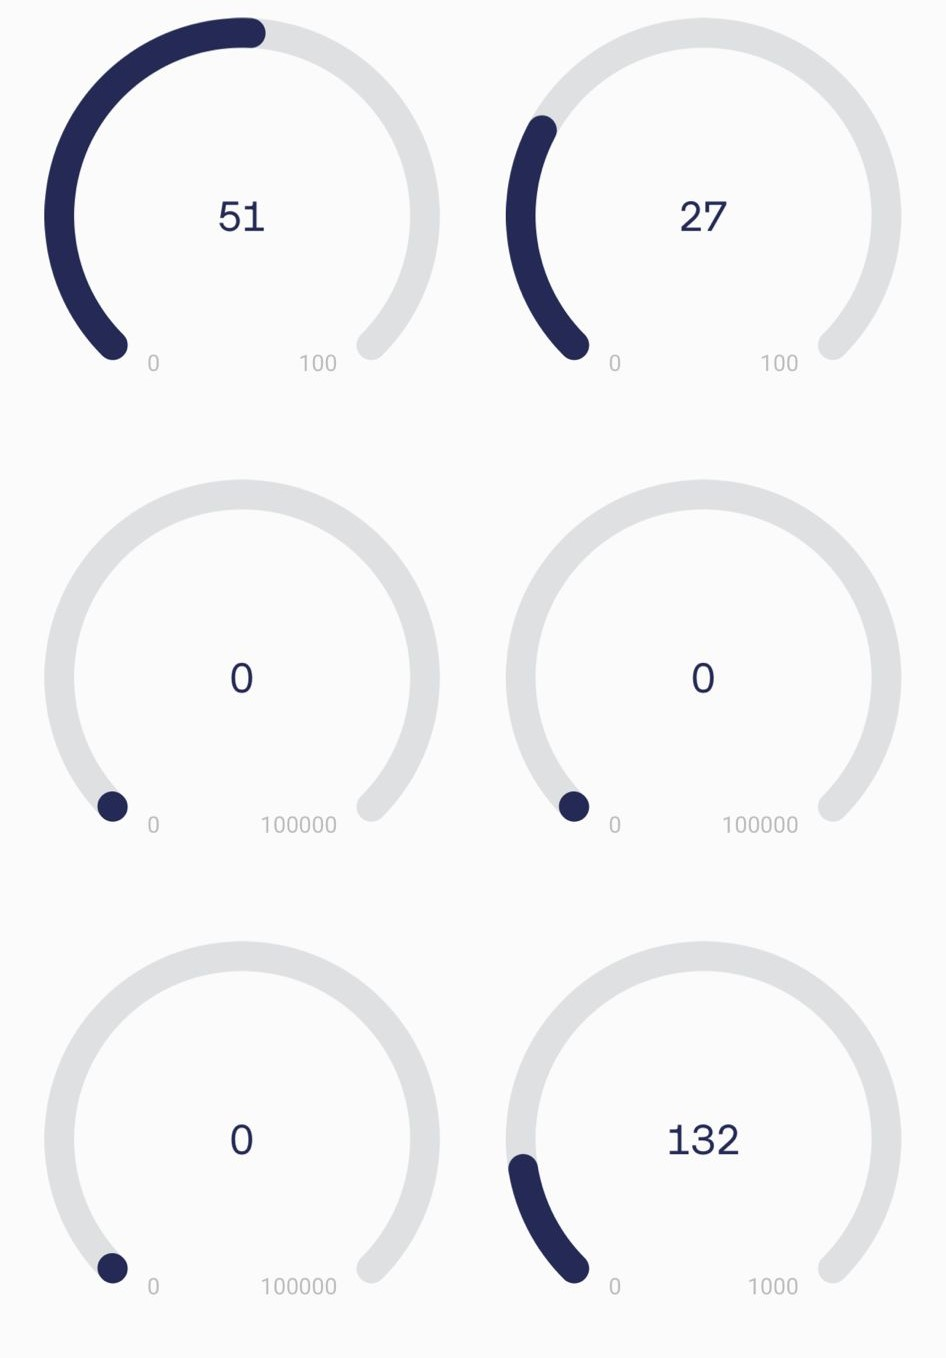
\includegraphics[width=0.4\linewidth]{bachelors_ro/images/interfata_blynk_mobile.jpg}
\caption{Interfața Mobile Blynk\cite{templ_blynk}}
\label{fig:interfata_blynk_mobile}
\end{figure}

\section{Transmiterea datelor către platforma Blynk}
După ce interfețele au fost configurate, următorul pas este trimiterea datelor prin WiFi către platforma Blynk. Pentru realizarea acestei transmisi avem nevoie de două biblioteci specifice: \texttt{ESP8266WiFi.h} \cite{lib_esp} și \texttt{BlynkSimpleEsp8266.h} \cite{lib_blynk}. Aceste biblioteci oferă posibilitatea de conexiune la WiFi a modulului și conectare la platforma Blynk.

Pentru a conecta modulul NodeMCU la dispozitivul creat pe platformă, avem nevoie de câteva informații cheie: id-ul template-ului, numele template-ului, cheia de autentificare, SSID-ul rețelei la care dorim să ne conectăm și parola acesteia. Acestea sunt transmise prin cod conform Fragmentului \ref{code:token_blynk} oferit de platforma Blynk \cite{blynk_browser}, însă au fost criptate din motive de securitate.

\begin{code}[H]
\begin{lstlisting}[language=C++]
#define BLYNK_TEMPLATE_ID           "TMPxxxxxx"
#define BLYNK_TEMPLATE_NAME         "Device"
#define BLYNK_AUTH_TOKEN            "AuthToken"

char ssid[] = "NetworkName";
char pass[] = "Password";
\end{lstlisting}
\caption{Declararea informațiilor pentru conectarea la dispozitivul Blynk \cite{blynk_browser}}
\label{code:token_blynk}
\end{code}

Apoi, pentru a inițializa conexiunea, în \texttt{setup()} este apelată funcția \texttt{Blynk.begin(BLYNK\_AUTH\_TOKEN, ssid, pass)}. Argumentele acesteia sunt datele declarate anterior și indică device-ul Blynk la care trebuie să ne conectăm și rețeaua pe care trebuie să o folosim. 

În urma conectării la rețea și la dispozitivul Blynk, datele decodificate de NodeMCU sunt trimise către pinii virtuali definiți în subcapitolul \ref{configurare_blynk}. În Fragmentul \ref{code:send_data_to_blynk} este prezentată metoda de transmitere a datelor. Funcția \texttt{Blynk.run()} asigură menținerea conexiunii și sincronizarea între modulul NodeMCU și platforma Blynk. Bucla \texttt{for} este iterată de 7 ori pentru fiecare valoare decodificată și pentru fiecare pin virtual. Cu ajutorul indexului \texttt{i} fiecărui pin virtual îi este desemnată o valoare decodificată folosind funcția \texttt{Blynk.virtualWrite()}. Acest ansamblu de cod se execută ciclic în funcția \texttt{loop()} și astfel transmiterea datelor de la NodeMCU la platforma web și mobile Blynk este realizată cu succes.

\begin{code}[H]
\begin{lstlisting}[language=C++]
Blynk.run();

for (int i = 0; i < 7; i++) {
    Blynk.virtualWrite(V0 + i, valuesFromSen[i]);
}
\end{lstlisting}
\caption{Trimiterea datelor către pinii vituali}
\label{code:send_data_to_blynk}
\end{code}
